The necropolix of Ramsey is a complex of underground mausoleums, buried by earth and time.
It is also where Dr. Jonas almost got fired.
After finding her first mummy, she seemed to be cursed.
Whenever she entered a new crypt, the mummy inside of it would be as far away from her team as possible.
It's not that they had a hard time finding the mummies, in fact the walls had directions on them leading straight to the sarcophagus.
Still, she had of run of impossibly bad luck.

Once the university realized how much resources Dr. Jonas was spending on her digs, they demanded she stop ``wasting'' their money.
She needed to minimize the number of rooms her team was exploring.
Using ground penetrating radar, Dr. Jonas was able to scout out possible sarcophagus locations and the passages between them.
For instance, one site looked like

\begin{center}
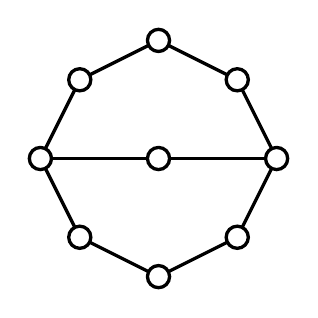
\begin{tikzpicture}[scale=0.5]
    \draw [very thick] (-3,0) -- (3,0);
    \draw [very thick] (-3,0) -- (-2,2) -- (0,3) -- (2,2) -- (3,0) -- (2,-2) -- (0,-3) -- (-2,-2) -- cycle;
    
    \filldraw [color = black, fill = white, very thick] (0,0) circle (8pt);
    \draw [color = black, fill = white, very thick] (-3,0) circle (8pt);
    \draw [color = black, fill = white, very thick] (3,0) circle (8pt);
    \draw [color = black, fill = white, very thick] (0,-3) circle (8pt);
    \draw [color = black, fill = white, very thick] (0,3) circle (8pt);
    \draw [color = black, fill = white, very thick] (2,2) circle (8pt);
    \draw [color = black, fill = white, very thick] (-2,2) circle (8pt);
    \draw [color = black, fill = white, very thick] (2,-2) circle (8pt);
    \draw [color = black, fill = white, very thick] (-2,-2) circle (8pt);
  \end{tikzpicture}
  \end{center}
  
where the circles represent rooms and the lines represent the passages connecting them.

Dr. Jonas could send 9 people out to the site and find the mummy immediately, but that's not very efficient.
Instead, she can send down just 2 people, and have the maximum number of rooms they have to explore be three 3.
Following the Univeristy accounting scheme, this has a cost of 5 as opposed to 9.
This is the best that Dr. Jonas can do.
\begin{center}
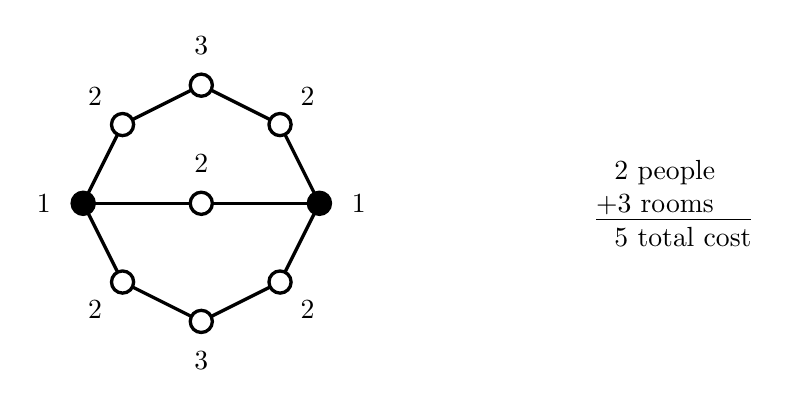
\begin{tikzpicture}[scale=0.5]
    \draw [very thick] (-3,0) -- (3,0);
    \draw [very thick] (-3,0) -- (-2,2) -- (0,3) -- (2,2) -- (3,0) -- (2,-2) -- (0,-3) -- (-2,-2) -- cycle;
    
    \draw [color = black, fill = white, very thick] (0,0) circle (8pt);
    \draw [color = black, fill = black, very thick] (-3,0) circle (8pt);
    \draw [color = black, fill = black, very thick] (3,0) circle (8pt);
    \draw [color = black, fill = white, very thick] (0,-3) circle (8pt);
    \draw [color = black, fill = white, very thick] (0,3) circle (8pt);
    \draw [color = black, fill = white, very thick] (2,2) circle (8pt);
    \draw [color = black, fill = white, very thick] (-2,2) circle (8pt);
    \draw [color = black, fill = white, very thick] (2,-2) circle (8pt);
    \draw [color = black, fill = white, very thick] (-2,-2) circle (8pt);

    \node at (0,1) {2};
    \node at (-4,0) {1};
    \node at (4,0) {1};
    \node at (0,-4) {3};
    \node at (2.7,2.7) {2};
    \node at (-2.7,2.7) {2};
    \node at (2.7,-2.7) {2};
    \node at (-2.7,-2.7) {2};
    \node at (0,4) {3};

    \node[align=left] at (12,0) {\,\, 2 people \\ \underline{+3 rooms \quad} \\ \,\, 5 total cost};
    
\end{tikzpicture}
\end{center}

There are four more site diagrams in Dr. Jonas' notes.
If you can figure out the minimum cost of exploring these crypts, B. Fraiser will be able to tell you how to deciper the next journal page.
